\chapter{Reti Neurali}
\section{Ai, Machine Learning, Deep Learning}

\begin{itemize}
    \item AI: Qualunque tecnica con cui una macchina può riprodurre il comportamento umano.
    \item Machine Learning: Qualunque tecnica con cui una macchina può svolgere compiti senza essere esplicitamente programmata, ma semplicemente imparando per esperienza precedente.
    \item Deep Learning: Una specifica tecnica di machine learning, che implementa l’apprendimento attraverso reti neurali artificiali.
\end{itemize}

\subsection{Apprendimento}
Possiamo dividere i tipi di Apprendimento in:
\begin{itemize}
    \item Apprendimento Non Supervisionato: vuol dire che i dati a disposizione sono soltanto i dati di input
    \item Apprendimento Supervisionato: vuol dire che i dati a disposizione sono i dati di input con i corrispettivi dati di output
\end{itemize}


\section{Apprendimento Supervisionato}
Supponiamo di avere i seguenti dati d'esempio:
\begin{center}
    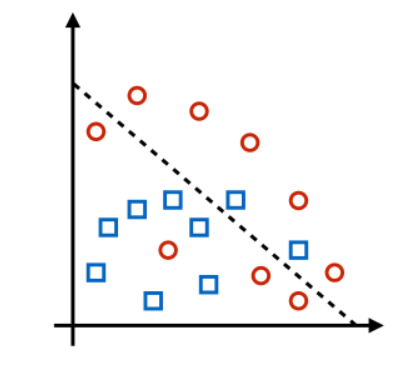
\includegraphics[width=\textwidth/2]{Images/SetEsempio.png}
\end{center}
Un Algoritmo di Learning imposta i Parametri di Progetto denotati con $\theta$, come la pendenza della retta.
\\
\begin{center}
    Ma come si impostano???
\end{center}
\subsection{Training Set}
Definendo il Training Set con $S_{TR}\{ (x_n, y_n^*)\}$ per $n=1,...,N_{TR}$, i parametri $\theta$ si impostano in modo tale da minimizzare:
\begin{equation*}
    \min_\theta \sum_{n=1}^{N_{TR}} \mathbb{L}(y_n(\theta), y_n^*)
\end{equation*}
dove:
\begin{itemize}
    \item $y_n$ è il risultato effettivo per l'ingresso $x_n$
    \item $\mathbb{L}$ è una funzione di errore
\end{itemize}
Oltre a $\theta$ un Algoritmo di Learning deve impostare altri parametri, che non possono essere impostati con il Training Test, ovvero gli Iperparametri, come la scelta di una curva anzichè un'altra.

\subsection{Validation Set}
Il Validation Set serve per testare l'algoritmo con dati non presenti nel Training Test, dato che lo scopo ultimo dell'algoritmo è la generalizzazione.

\subsection{Test Set}
Il Test Set svolge lo stesso ruolo del Validation Set, per questo lo scopo dell'algoritmo non è minimizzare l'errore nel training, ma è minimizzare l'Error Test.

\subsection{Overfitting e Uderfitting}
Si ha Overfitting quando l'algoritmo di Learning si specializza troppo sul training set in uso.\\ \\

Si ha Underfitting quando si ha un Errore Medio sul Training Set troppo basso.\\ \\
\begin{center}
    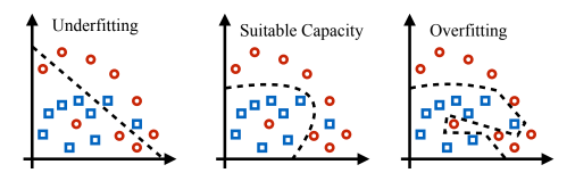
\includegraphics[width=\textwidth]{Images/UnderfittingOverfitting.png}
\end{center}


\section{Deep Learning}
Il Deep Learning utilizza, nel processo di apprendimento, le Reti Neurali Artificiali (ANN).\\ \\
Le ANN sono organizzare in Layer, composti da "neuroni", divisi in:
\begin{itemize}
    \item Input Layer che prendono i dati in ingresso e li inoltrano al Layer successivo
    \item Hidden Layer è il Layer che elabora i dati
    \item Output Layer che elabora i dati prima di mandarli in output
\end{itemize}

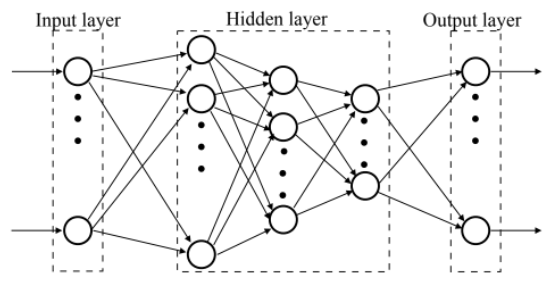
\includegraphics[width=0.8\textwidth]{Images/ANNmodel.png}
\subsection{Classificazioni delle ANN}
Le ANN possono essere classificate in:
\begin{itemize}
    \item Feedforward Neural Network (FNN) \\in cui i dati si propagano in una sola direzione
    \begin{itemize}
        \item Fully-Connected Neural Network (FCNN) \\è un caso particolare delle FNN, in cui ciascun neurone è connesso a tutti i neuroni del Layer successivo
        \item Convolutional Neural Network (CNN) \\è una  FNN in cui ogni neurone fa una convoluzione dell'ingresso
    \end{itemize}
    \item Recurrent Neural Network (RNN) \\è una ANN in cui sono permessi loop, quindi l'uscita di un neurone potrebbe essere messa in ingresso ad un Layer precedente
    
    \item Deep Neural Network (DNN) \\è una ANN con più di un Hidden Layer
    \item Shallow Neural Network (SNN) \\è una ANN con un solo Hidden Layer
\end{itemize}



\section{Fully-Connected Neural Network}
Nelle FCNN l'ingresso del k-esimo layer è un vettore $\vc{x}_{k-1}$.\\ \\
Mentre l'uscita dell'i-esimo neurone del k-esimo Layer sarà:
\begin{equation*}
\begin{aligned}
    x_k (i) = f_{i,k} (z_{i,k}) \\
    z_{i,k} = \vc{w}_{i,k}^T \vc{x}_{k-1} + b_{i,k}
\end{aligned}
\end{equation*}\\
dove:
\begin{itemize}
    \item $\vc{w}_{i,k}$ è un vettore di Pesi
    \item $b_{i,k}$ è un termine di Bias
    \item $f_{i,k} (z_{i,k})$ è una Funzione di Attivazione
\end{itemize}

\subsection{Funzioni di Attivazione}
Qualsiasi funzione può essere usata come Funzione di Attivazione, tuttavia esistono alcune scelte canoniche come la funzione Lineare, che viene usata al più dal Layer di Output e le funzioni Sigmoidali e Iperboliche, che non sono quasi mai usate per la loro difficile applicazione.\\ \\
Le funzioni più largamente usate sono:
\begin{itemize}
    \item Rectified Linear Unit (ReLU) è la più diffusa, anche se presenta il problema che sia identicamente nulla per ingressi negativi:
    \begin{equation*}
        ReLU(z_{i,k}) = max(0, z_{i,k})
    \end{equation*}
    \item Generalized ReLU, risolve il problema visto sopra:
    \begin{equation*}
        G-ReLU(z_{i,k}) = max(0, z_{i,k}) + c \cdot min(0, z_{i,k})
    \end{equation*}
    \item Exponential Linear Unit (ELU) risolve lo stesso problema, ma pone gli ingressi negativi come esponenziali:
    \begin{equation*}
        E-ReLU(z_{i,k}) = \begin{cases}
        \alpha (e^{z_{i,k}} -1) & z_{i,k} \leq 0 \\
        z_{i,k} & z_{i,k} > 0
        \end{cases}
    \end{equation*}
\end{itemize}



\section{Convolutional Neural Network}
\subsection{Layer Convoluzionali}
Nelle Reti Convoluzionali, in ingresso si ha una matrice 3D, di dimensioni N X N X $N_c$\\ \\
Ad ogni neurone è associato un Filtro indicato con \vc{W} di dimensioni F X F X $N_{c,f}$ ($F \leq N$) quindi più piccolo della matrice di Input.\\ \\
Ogni neurone esegue una Cross-Correlazione a Finestra Mobile\footnote{Nel gergo delle ANN con un abuso di notazione viene chiamato Convoluzione}\\ \\
Il risultato sarà una matrice 2D \vc{Y}, con dimensioni N - F + 1 X N - F + 1

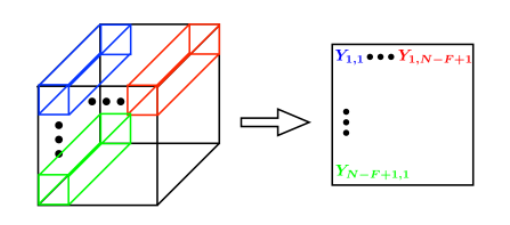
\includegraphics[width=0.8\textwidth]{Images/Convolutional.png}

Alla matrice \vc{Y} sommeremo un termine di Bias per ogni neurone ed una Funzione di Attivazione per ogni componente di \vc{Y}.\\ \\

Tutte le matrici \vc{Y} del Layer vengono unite per formare una matrice 3D di dimensioni (N - F - 1) X (N - F - 1) X $N_F$  ed inoltrate in ingresso al Layer successivo.

\subsection{Pooling Layer}
Il Pooling è un'operazione svolta da un intero Layer, operando su ogni "strato"\footnote{Sugli $N_{F_i}$} della matrice di Input:
\begin{center}
    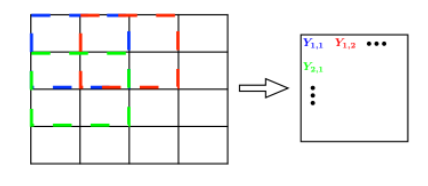
\includegraphics[width=0.8\textwidth]{Images/Pooling.png}
\end{center}

\subsubsection{Max Pooling}
Per ogni "strato" della matrice di Input, seleziona il massimo tra gli elementi di ogni sotto-matrice di dimensione F X F.

\subsubsection{Average Pooling}
Per ogni "strato" della matrice di Input, seleziona la media tra gli elementi di ogni sotto-matrice di dimensione F X F.



\section{Addestramento di Reti Neurali Artificiali}
\subsection{ANN Training}
Dato il Training-Set:
\begin{equation*}
    S_{TR} = \{x_n, y_n^*\}, n=1,...,N_{TR}
\end{equation*}
l'obbiettivo dell'Algoritmo di Learning è quello di OTTIMIZZARE l'assegnazione dei Pesi e dei Coeficienti di Bias contenuti in una variabile $\theta$:
\begin{equation*}
    \min_\theta \sum_{n=1}^{N_{TR}} \mathbb{L}(y_n(\theta), y_n^*)
\end{equation*}
Per risolvere questo problema si utilizzano metodi come l'Algoritmo del Gradiente.

\subsection{Algoritmo del Gradiente}
L'Algoritmo del Gradiente ha lo scopo di minimizzare una funzione.\\ \\
Consideriamo il seguente problema:
\begin{equation*}
    \min_{\vc{x}} f(\vc{x})
\end{equation*}
Il Gradiente indica la direzione di massimo incremento della funzione, quindi l'algoritmo si muoverà in senso opposto rispetto al gradiente per trovare il minimo.



\begin{algorithm}
\caption{Algoritmo del Gradiente}
\begin{algorithmic}
\Ensure {Inizializza} $x_{new}, \alpha >0, \epsilon >0$ \Comment{$\alpha$ viene detto step-size}
\Repeat
\State $\vc{x}_{old} = \vc{x}_{new}$
\State $\vc{x}_{new} = \vc{x}_{old} - \alpha \nabla f(\vc{x}_{old})$
\Until{$||\vc{x}_{new} - \vc{x}_{old}|| < \epsilon$}
\end{algorithmic}
\end{algorithm}
L’algoritmo del gradiente converge ad un Punto Stazionario ($\nabla f = 0$) per $\alpha$ opportuni.\\ \\
Tuttavia con $\alpha$ non opportunamente scelti si potrebbe cadere in uno di questi due casi:
\begin{center}
    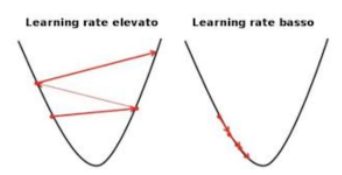
\includegraphics[width=0.6\textwidth]{Images/AlfaInopportuni.png}

IMPORTANTE: \\L'Algoritmo del Gradiente arriva ad un Punto Stazionario, che NON è detto che sia un Minimo Globale!!\\
Ma non è detto che sia un problema, perchè alle volte trovare un Minimo Globale causerebbe un Overfitting!!!
\end{center}

\subsection{Metodo del Gradiente Stocastico}
L'Algoritmo del Gradiente è troppo complesso da calcolare per grandi quantità di dati.\\ \\
Quindi scriviamo il Gradiente del Training-Set:
\begin{equation*}
    \nabla_{\theta} \ \Delta_{TR}(\theta) = \sum_{n=1}^{N_{TR}} \nabla_{\theta} \ \mathbb{L}(y_n (\theta), y_n^*)
\end{equation*}
Ed ora calcoliamo un'approssimazione del Gradiente, su un sotto-insieme S del Training-Set, chiamato mini-batch, con $N << N_{TR}$:
\begin{equation*}
    \widehat{\nabla_{\theta} \ \Delta_{TR}(\theta)} = \sum_{n \in S} \nabla_{\theta} \ \mathbb{L}(y_n (\theta), y_n^*)
\end{equation*}
\subsubsection{SGD Training Algorithm}
\begin{algorithm}
\caption{SGD Training Algorithm}
\begin{algorithmic}
\Ensure {Inizializza} $\vc{W},\vc{b}$
\Repeat
\State $\text{Selezionare un mini-batch a caso chiamandolo S}$
\State $\text{Calcola } \widehat{\nabla_{\theta} \ \Delta_{TR}(\theta)} $
\State $\vc{W} = \vc{W} - \alpha \widehat{\nabla \Delta_{TR}}(\vc{W},\vc{b}), \text{con } \vc{b} = \vc{b} - \alpha \widehat{\nabla \Delta_{TR}}(\vc{W},\vc{b})$
\Until{$\text{Controlla la convergenza}$}
\end{algorithmic}
\end{algorithm}


\section{Regolarizzazione}
Ogni metodo che minimizza il Test Error, a discapito del Training Error (quindi cerca di evitare l'Underfitting) viene detto metodo di Regolarizzazione, che possiamo suddividere in varie categorie.
\subsection{Regolarizzazione $L^P$}
Consiste nel "perturbare" la funzione di costo usata per il Training aggiungendo la norma $L^P$:
\begin{equation*}
    \Delta_r (\vc{W},\vc{b}) = \Delta_{TR}(\vc{W},\vc{b}) + \phi ||\vc{W}||_p^p
\end{equation*}
dove $\phi$ è un Iper Parametro che indica il peso della "perturbazione".\\

Da qui specificando si possono ottenere le definizioni di Regolarizzazione $L^2$ e $L^1$.
\subsubsection{Early Stopping}
L'Early Stopping consiste nell'interrompere il Training quando il Validation Error non è diminuito per T iterazioni di Training.

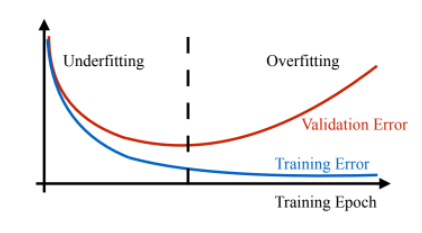
\includegraphics[width=0.8\textwidth]{Images/EarlyStopping.png}